\chapter{MTD子系统分析}
\section{MTD简介}
MTD,Memory Technology Device即内存技术设备,MTD的存在屏蔽了flash驱动实现细节,向上(主要指文件系统)提供统一的API接口。并且MTD只能工作在raw flash上,目前市面上主要有以下几种类型的flash
\begin{itemize}
  \item raw flash,原始flash设备,采用ONFI接口,只有基本的存储功能 。不提供ecc除错,坏块管理,负载均衡等机制,这些都是由host processor提供
  \item clear flash,将ECC机制整合进了flash芯片中的新型flash,采用ONFI接口
  \item emmc,将nand flash与控制芯片封装在一起,提供了ECC除错,坏块管理,负载均衡等机制,采用JEDEC标准 
  \item UFS,通用flash存储器,具备emmc功能,并且可以读写数据同时进行,采用JEDEC标准
\end{itemize}

\section{MTD驱动结构}
MTD向用户空间提供了字符设备节点与块设备节点供用户空间程序直接操作flash设备,向文件系统提供了MTD原始设备层,文件系统不再关心flash驱动具体实现

\begin{figure}[htbp]
\centering
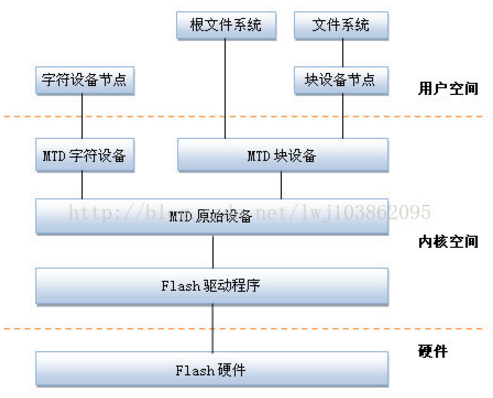
\includegraphics[keepaspectratio,width=0.5\textwidth,height=0.24\textheight]{img/mtd_struct.png}
\end{figure}
在上图中可以发现,MTD原始设备是对NandFlash封装的一层。下面主要分析原始设备层是如何使用NandFlash驱动,以及向上层提供了哪些封装函数。下面简单介绍一下MTD驱动目录下各个文件的用处:
\begin{mdframed}[backgroundcolor=lightgray,hidealllines=true]
\dirtree{%
.1 mtd/.
.2 nand/.
.3 nand\_base.c\DTcomment{里面定义了大量MTD框架所需的默认函数,flash读/写/擦除/ECC/BBT/等}.
.3 nand\_bbt.c\DTcomment{MTD坏块与坏块表管理}.
.3 nand\_ecc.c\DTcomment{实现Hanming ECC默认的ecc code计算函数与较正函数(calculate与correct)}.
.3 nand\_bch.c\DTcomment{实现BCH ECC默认的计算与较正函数}.
.3 s3c2410.c\DTcomment{s3c2410平台flash具体操作实现,如果不实现则使用nand\_base中默认函数}.
.2 mtd\_char.c\DTcomment{与MTD相关的char,block,class,proc等注册的地方,并向外界提供获取mtd的方法}.
.2 mtd\_core.c\DTcomment{MTD向应用层提供的块设备驱动}.
.2 mtd\_block.c\DTcomment{MTD向应用层提供的块设备驱动}.
.2 mtdpart.c\DTcomment{mtd分区相关,定义mtd分区的mtd\_info结构所需的各种参数与回调函数}.
}
\end{mdframed}

\section{MTD原始设备层}
操作NandFlash主要有三个动作,读/写/擦除。MTD原始设备在read/write/erase函数中会调用nand flash chip驱动的相应操作方法,而文件系统则可以直接使用原始设备层提供的read/write/erase去操作flash。
%\clearpage
\subsection{主要数据结构分析}
struct mtd\_info就代表MTD原始设备层,这个结构体的函数是需要驱动开发人员实现的,实现这些函数比较简单,基本都是直接调用nand flash驱动的函数。
\begin{lstlisting}[language=C]
struct mtd_info {
	u_char type; //nor flash or nand flash(mlc/slc/tlc)
	uint32_t flags; //mtd-abi.h中定义它的属性值
	uint64_t size; //mtd设备大小,就是分区大小
	uint32_t erasesize; //block大小
	uint32_t writesize; //最小写单位,对于nandflash就是PageSize(或subPageSize)
	uint32_t writebufsize; //基本未使用,writebufsize可以减少向flash写入次数
	uint32_t oobsize; //OOB字节数,spare space size
	uint32_t oobavail; //可用OOB字节数
	unsigned int erasesize_shift; //默认0
	unsigned int writesize_shift; //默认0
	unsigned int erasesize_mask;  //默认0
	unsigned int writesize_mask;  //默认0
	unsigned int bitflip_threshold; //bitflip数超过这个值,就会报EUCLEAN错误,这个值可以通过sysfs修改
	const char *name; //mtd名字,一般就是分区名cat /proc/mtd读出来的
	int index; //idr机制产生,挂在全局mtd_idr上,可以直接通过index找到slave mtd_info(后面用到)
	struct nand_ecclayout *ecclayout; //ecc在oob中布局,根据硬件得到
	unsigned int ecc_step_size; //一次对多少字节进行校验计算,一般是256或512字节
	unsigned int ecc_strength; //可校准bitflip位数
	int numeraseregions; //不同的erasesize区域数目,通常都是1
	struct mtd_erase_region_info *eraseregions;
	int (*_erase) (struct mtd_info *mtd, struct erase_info *instr); //块擦除函数,实现时会跳坏块
	... ...
	int (*_read) (struct mtd_info *mtd, loff_t from, size_t len,
		      size_t *retlen, u_char *buf); //读page函数
	int (*_write) (struct mtd_info *mtd, loff_t to, size_t len,
		       size_t *retlen, const u_char *buf); //写page函数
	int (*_panic_write) (struct mtd_info *mtd, loff_t to, size_t len,
			     size_t *retlen, const u_char *buf);
	int (*_read_oob) (struct mtd_info *mtd, loff_t from,
			  struct mtd_oob_ops *ops); //带oob读函数
	int (*_write_oob) (struct mtd_info *mtd, loff_t to,
			   struct mtd_oob_ops *ops); //带oob写函数
	... ...
	void (*_sync) (struct mtd_info *mtd);
	int (*_lock) (struct mtd_info *mtd, loff_t ofs, uint64_t len); //nandflash支持设备独占访问时定义
	int (*_unlock) (struct mtd_info *mtd, loff_t ofs, uint64_t len);//nandflash解锁
	int (*_is_locked) (struct mtd_info *mtd, loff_t ofs, uint64_t len);
	int (*_block_isreserved) (struct mtd_info *mtd, loff_t ofs);
	int (*_block_isbad) (struct mtd_info *mtd, loff_t ofs); //坏块判断函数
	int (*_block_markbad) (struct mtd_info *mtd, loff_t ofs); //使用中出现坏块时的标记函数
	int (*_get_device) (struct mtd_info *mtd);
	void (*_put_device) (struct mtd_info *mtd);
	struct backing_dev_info *backing_dev_info;
	struct notifier_block reboot_notifier;
	struct mtd_ecc_stats ecc_stats; //ecc较验统计,坏块数量,较验次数等
	void *priv; //mtd_info私有数据,通常指向nand_chip结构体
	struct device dev;
	int usecount;
};

\end{lstlisting}

\clearpage

struct nand\_chip结构体代表的是flash驱动,它是直接与硬件通信的,因此nand\_chip中的需要用到的函数都是由驱动开发人员实现。nand chip也不必使用MTD自带的struct nand\_chip,驱动开发自己定义,然后自己实现也是可以的,高通自定义的为struct msm\_nand\_chip。
\begin{lstlisting}[language=C]
struct nand_chip {
	void __iomem *IO_ADDR_R; //读/写8根IO线的地址
	void __iomem *IO_ADDR_W;
	/* 从nand flash控制器的寄存器中读一字节 */
	uint8_t (*read_byte)(struct mtd_info *mtd);
	/* 从nand flash控制器的寄存器中读一个字,默认是2个字节 */
	u16  (*read_word)(struct mtd_info *mtd); 
	/* 写一字节到nand flash控制器的寄存器中 */
	void (*write_byte)(struct mtd_info *mtd, uint8_t byte);
	/* 将缓冲区内容写入nand flash中 */
	void (*write_buf)(struct mtd_info *mtd, const uint8_t *buf, int len); 
	/* 将nand flash内容读到缓冲区 */
	void (*read_buf)(struct mtd_info *mtd, uint8_t *buf, int len); 
	/* chip片选,一般有多个nand flash芯片时会用到 */
	void (*select_chip)(struct mtd_info *mtd, int chip); 
	/* 读指定块的坏块标记,确认它是不是坏块 */
	int  (*block_bad)(struct mtd_info *mtd, loff_t ofs, int getchip); 
	/* 标记一个块为坏块,向待标记块的flash oob区写入坏块信息 */
	int  (*block_markbad)(struct mtd_info *mtd, loff_t ofs); 
	/* 向nand flash控制器的cmd寄存器(使能芯片,启动ecc等)写入控制信息 */
	void (*cmd_ctrl)(struct mtd_info *mtd, int dat, unsigned int ctrl);
	/* 初始化flash容量信息,包括PageSize,OOBSize,EraseSize等信息 */
	int  (*init_size)(struct mtd_info *mtd, struct nand_chip *this, u8 *id_data);
	/* 从nand flash控制器的寄存器中获取设备当前状态,Busy or Ready */
	int  (*dev_ready)(struct mtd_info *mtd);
	/* 向nand flash发送命令,复位chip,擦除block,读flash等 */
	void (*cmdfunc)(struct mtd_info *mtd, unsigned command, int column, int page_addr);
	/* 等待命令完成,主要用于nand flash的写入与擦除两个动作 */
	int  (*waitfunc)(struct mtd_info *mtd, struct nand_chip *this);
	/* nand chip实现的擦除函数,这个函数可以擦除所有块,包括坏块 */
	int  (*erase)(struct mtd_info *mtd, int page);
	/* 扫描坏块,创建坏块表,坏块表是为了加快坏块查找速度 */
	int  (*scan_bbt)(struct mtd_info *mtd);
	/* 硬件功能,对错误码进行判断,看是否可以较正*/
	int (*errstat)(struct mtd_info *mtd, struct nand_chip *this, int state,
		int status, int page);
	/* 设置ONFI nand特性 */
	int (*onfi_set_features)(struct mtd_info *mtd, struct nand_chip *chip,
			int feature_addr, uint8_t *subfeature_para);
	/* 获取ONFI nand特性 */
	int (*onfi_get_features)(struct mtd_info *mtd, struct nand_chip *chip,
			int feature_addr, uint8_t *subfeature_para);
	/* 设置nand flash重读模式,一般MLC flash是需要设置的 */
	int (*setup_read_retry)(struct mtd_info *mtd, int retry_mode);
	
	int chip_delay;
	unsigned int options;
	/*
	 * NAND_BBT_USE_FLASH:坏块表存在flash中,内核可以直接读出
	 * NAND_BBT_SCANLASTPAGE:
	 */
	unsigned int bbt_options; //坏块表创建操作选项,它的取值定义在bbm.h中
	int page_shift; //一个page占用的地址位数
	int phys_erase_shift; //一个PEB占用的地址位数
	int bbt_erase_shift; //bbt入口地址占用的位数,用来寻找bbt表
	int chip_shift; //芯片地址占用位数,一般不用
	int numchips; //共有多少个flash芯片,一般为1
	uint64_t chipsize;
	int pagemask; //页地址掩码
	int pagebuf; //当前保存在data buf中的page编号
	unsigned int pagebuf_bitflips; //当前读出的page产生的bitflip数量
	int subpagesize; //子页大小
	uint8_t bits_per_cell; //标记flash层数,mlc,tlc,slc等
	uint16_t ecc_strength_ds; //ecc可修正的位数,数据来源于datasheet,如果没有设为0
	uint16_t ecc_step_ds; //ecc一次可以较验多少字节的数据,从datasheet中获取
	int onfi_timing_mode_default;
	int badblockpos; //坏块标记在oob中的位置
	int badblockbits;
	union {
		struct nand_onfi_params	onfi_params;
		struct nand_jedec_params jedec_params;
	};
	int read_retries; //read retry mode支持的重读次数
	flstate_t state; //nand flash设备当前状态
	uint8_t *oob_poi; //写oob之前,先保存oob数据
	struct nand_hw_control *controller;
	struct nand_ecc_ctrl ecc; //与ECC相关的控制结构体,下面详解
	struct nand_buffers *buffers; //write/read时使用的buf
	struct nand_hw_control hwcontrol;
	uint8_t *bbt; //坏块表在内存中地址
	struct nand_bbt_descr *bbt_td; //坏块表描述符,描述一个块是否装有坏块表
	struct nand_bbt_descr *bbt_md; //坏块表描述符镜像
	struct nand_bbt_descr *badblock_pattern; //用于判断一个块是否是坏块,它的pattern是0xff
	void *priv; //nand chip私有数据
};

\end{lstlisting}
Nand flash比较容易发生bit flip错误,为了降低bit flip带来的影响,需要在nand读写时加入ecc较验,而带ecc的读写都是放在struct nand\_ecc\_ctrl中的,它会调用nand chip的读写函数,然后再使用ECC去较验读出的数据。
\begin{lstlisting}[language=C]
struct nand_ecc_ctrl {
	nand_ecc_modes_t mode; //ECC模式,软件ECC,硬件ECC等
	int steps; //一个nand flash page需要较验几次
	int size; //ECC一次较验多少字节
	int bytes; //每次较验,ECC较验码占多少字节
	int total; //一个nand flash page ECC较验占用多少字节 
	int strength; //一次ECC较验可以较正的位数
	int prepad;
	int postpad;
	struct nand_ecclayout	*layout; //ecc在oob中的布局
	void *priv; //ecc ctrl的私有数据,一般指向nand_bch_control
	void (*hwctl)(struct mtd_info *mtd, int mode); //控制硬件ECC产生,一般是enable硬件ecc模块
	int (*calculate)(struct mtd_info *mtd, const uint8_t *dat,
			uint8_t *ecc_code); //计算dat产生的ecc较验码,并通过ecc_code返回
	int (*correct)(struct mtd_info *mtd, uint8_t *dat, uint8_t *read_ecc,
			uint8_t *calc_ecc); //用calculate产生的ecc code与oob中的ecc code进行数据较验
	int (*read_page_raw)(struct mtd_info *mtd, struct nand_chip *chip,
			uint8_t *buf, int oob_required, int page); //原始读,不带ecc较验
	int (*write_page_raw)(struct mtd_info *mtd, struct nand_chip *chip,
			const uint8_t *buf, int oob_required); //原始写,不带ecc较验
	int (*read_page)(struct mtd_info *mtd, struct nand_chip *chip,
			uint8_t *buf, int oob_required, int page); //带ecc读,返回max-bitflip
	int (*read_subpage)(struct mtd_info *mtd, struct nand_chip *chip,
			uint32_t offs, uint32_t len, uint8_t *buf, int page);
	int (*write_subpage)(struct mtd_info *mtd, struct nand_chip *chip,
			uint32_t offset, uint32_t data_len,
			const uint8_t *data_buf, int oob_required);
	int (*write_page)(struct mtd_info *mtd, struct nand_chip *chip,
			const uint8_t *buf, int oob_required); //写入数据后,把数据的ecc较验码也写进去
	int (*write_oob_raw)(struct mtd_info *mtd, struct nand_chip *chip,
			int page);
	int (*read_oob_raw)(struct mtd_info *mtd, struct nand_chip *chip,
			int page);
	int (*read_oob)(struct mtd_info *mtd, struct nand_chip *chip, int page); //读oob区
	int (*write_oob)(struct mtd_info *mtd, struct nand_chip *chip,
			int page); //写oob区
};

\end{lstlisting}

上面主要介绍了MTD架构主要的几个结构体,struct mtd\_info是MTD原始设备层代表,它服务于mtd(mtdcore.c)核心层,mtd核心层向外部提供MTD API。struct nand\_ecc\_ctrl向mtd提供带ECC检验的读写方法,但mtd使用与否,则与mtd的读写函数的ops(ops->mode取MTD\_OPS\_RAW值时,不使用带ECC较验的读写)参数值相关。struc nand\_chip定义了直接操作硬件的方法,是flash的原始读写

\subsection{MTD初始化流程}
上面介绍的是接口类,是MTD架构中通用的东西,但涉及MTD具体使用时,是必须考虑平台的,这里以s3c2410与高通9x07平台为例,s3c2410是比较规范的按照MTD框架来写驱动程序,比较适合于学习MTD驱动框架。
\begin{mdframed}[style=leftredline]
\begin{verbatim}
--s3c24xx_nand_probe() //这是s3c24xx平台的Nand驱动开始的地方,probe函数原理参看linux设备驱动模型
----s3c2410_nand_init_chip() //对nand_chip,nand_ecc_ctrl结构体里的回调函数,数据进行初始化赋值
----nand_scan_ident() //扫描nand device有多少,记录数目和它们的容量大小
----nand_scan_tail() //nand_scan最后的扫描,主要对ecc相关函数进行赋值,并且在最后会扫描坏块表
----s3c2410_nand_add_partition() //建立mtd分区,下面描述
\end{verbatim}
\end{mdframed}
MTD驱动架构的存在简化上层开发者的工作量,MTD初始化流程也是对MTD框架的内容进行填充,在nand\_base.c文件中有很多MTD默认函数,s3c2410初始化nand flash过程中,如果s3c2410\_nand\_init\_chip中未定义的MTD函数,都会在nand\_base.c中获得一个默认的操作函数。

\subsection{MTD分区建立}
MTD分区建立后,每个分区都有一个mtd\_info结构体,原先的mtd\_info称为master,分区的mtd\_info称为slave,它们的回调函数指向是不同的,但slave mtd\_info最终一定会调用master mtd\_info。分区建立需要一个输入,就是分区表。内核需要获取到分区表之后才能划分MTD分区,分区表传递给内核的方法很多,其中包括早期内核使用的mach文件,现在的设备树文件,以及把分区表以bin形式下载到nand flash中,bootloader解析之后通过cmdline或共享内存的方法传递给内核。
\begin{lstlisting}[language=C]
struct mtd_partition {
	char *name; //分区名字,cat /proc/mtd可以看到
	uint64_t size;	//分区大小
	uint64_t offset; //分区偏移量,相对于flash 0地址的偏移
	uint32_t mask_flags; //可以设置成MTD_WRITEABLE变成只读分区
	struct nand_ecclayout *ecclayout; //分区的ECC布局
};
\end{lstlisting}
分区表的划分就是根据mtd\_partition结构体来的,填充多少个这样的结构体就会产生多少个分区,可以说mtd\_partition就是分区表。分区表获取,分区注册过程如下(以s3c2410为例,其它平台类似):
\begin{mdframed}[style=leftredline]
\begin{verbatim}
--s3c2410_nand_add_partition() //这个函数会简单处理一下注册的参数
----mtd_device_parse_register() //它的types参数决定它用什么方法解析分区表
------parse_mtd_partition() //解析分区表,并将解析内容填充到mtd_partition结构体中
----add_mtd_partitions() //创建并填充slave mtd_info,然后进行mtd_info注册(它的输入参数是mtd分区表)
------add_mtd_device() //mtd设备注册,并同时注册char,block等设备
\end{verbatim}
\end{mdframed}
分区表解析函数分析过程如下:
\begin{lstlisting}[language=C]
/*
 * mtd: master mtd_info,分区的mtd_info很多参数都是自于master mtd_info
 * types: 决定parse_mtd_partitions将调用哪个解析方法来解析,设NULL,则采用默认参数
 * parts: 是未调用系统解析方法输入进去的参数,如果系统方法解析失败,就使用parts分区表。
 * part参数的存在,使得MTD分区表解析更加多样化,例如高能平台就是在bootloader阶段解析后
 * 通过bootloader与kernel共享内存的方法把分区表传给内核,高通平台在MTD初始化阶段把它解析
 * 后放在parts中。
 */
int mtd_device_parse_register(struct mtd_info *mtd, const char * const *types,
			      struct mtd_part_parser_data *parser_data,
			      const struct mtd_partition *parts,
			      int nr_parts)
{
	int err;
	struct mtd_partition *real_parts; //真实分区表,需要当作参数传给add_mtd_partitions
	/*根据types类型去调用系统方法解析分区表,types默认的类型是cmdline与ofpart(设备树)*/
	err = parse_mtd_partitions(mtd, types, &real_parts, parser_data);
	if (err <= 0 && nr_parts && parts) {
		real_parts = kmemdup(parts, sizeof(*parts) * nr_parts,
				     GFP_KERNEL);//如果系统解析失败且parts存在,就使用parts分区表
		if (!real_parts)
			err = -ENOMEM;
		else
			err = nr_parts;//这时的err的值表示的是分区数量
	}
	if (err > 0) {
		err = add_mtd_partitions(mtd, real_parts, err);//根据分区表完成MTD分区注册
		kfree(real_parts);
	} else if (err == 0) {
		err = add_mtd_device(mtd);
		if (err == 1)
			err = -ENODEV;
	}
	return err;
}
\end{lstlisting}

\section{MTD设备层}
MTD设备层已经导出到用户空间,上层应用可以通过MTD字符设备与块设备来对flash进行访问。MTD字符设备提供了很多丰富的功能,包括获取MTD设备信息,坏块的判断,ECC状态获取等
\subsection{MTD字符设备}
MTD字符设备节点类似于/dev/mtd0(主设备号为90)这样,应用可以直接调用open/read/write/ioctl等系统调用来操作这个MTD的字符设备。下面来分析一下在内核空间,MTD为字符设备提供了哪些服务
\begin{lstlisting}[language=C]
/* mtd_fops是mtd char device的文件操作函数,对于不同的MTD分区,它们的字符设备主设备号都是90。
 * 因此它们的驱动是相同的,也就是共有mtd_fops。它们的次设备号不同,次设备决定它们的设备文件是什么
 */
static const struct file_operations mtd_fops = {
	.llseek		= mtdchar_lseek,//提供对flash分区地址定位
	.read		= mtdchar_read,//开始读flash,字节读(事实是读一个page,上传一个字节而已)
	/* write操作需要size参数page对齐,否则会返回无效参数的错误。nand flash的特点是先擦除,
	 * 后写入,所以不能对flash进行覆盖写。MTD提供了擦除操作,也提供了写入操作,但并不会在
	 * 写入之前进行flash是否擦除的检查,这就需要文件系统来做写入前是否擦除的保证
	 */
	.write		= mtdchar_write,
	/* ioctl的command定义在mtd_abi.h(内核空间),用户空间mtd-untils工具集中也在mtd_abi.h中
	 * MEMGETINFO:获取mtd信息(推荐使用sysfs读取mtd信息)
	 * MEMERASE:擦除指定块
	 * MEMGETBADBLOCK:判断指定块是否是坏块
	 * ECCGETSTATS:可以获取ECC状态,以及当前坏块数量等信息
	 */
	.unlocked_ioctl	= mtdchar_unlocked_ioctl,
	.open		= mtdchar_open, //mtd_file_info初始化
	.release	= mtdchar_close,
	.mmap		= mtdchar_mmap, //上层应用进行mmapj映射
	.get_unmapped_area = mtdchar_get_unmapped_area,
};
\end{lstlisting}

\section{MTD坏块管理}
严格来说,MTD是不具备坏块管理功能的,它只是向文件系统或应用程序提供了坏块判断,坏块信息写入OOB以及坏块表管理等机制。因此可以说MTD是坏块管理机制的实现者,而不是坏块管理策略的实现者。例如,对于UBI来说,它是具备坏块管理功能的,通过UBIFS来读写flash是不需要关注是否有坏块的。
\subsection{坏块判断}
mtdcore向外提供了接口:mtd\_block\_isbad(struct mtd\_info *mtd, loff\_t ofs),这个函数是模块符号导出函数,只需要给出分区slave mtd\_info和指定块偏移就可以了,返回值非0是坏块。而这个函数会调用mtd->\_block\_isbad,所以驱动开发者需要实现这个回调函数。具体的坏块判断是读出指定block第一个page的oob区域第1与第2字节是否是0xff(不同平台可能OOB偏移会不同,原理相同),如果不是0xff则是坏块。(为了加快坏块判断速度,内核提供了坏块表功能,在MTD初始化时扫描nand flash所有坏块,把坏块块信息加入坏块表中。如果要查询坏块,只要先在坏块表中查询,查询不到才使用读OOB方法)。
\subsection{坏块表建立}
MTD坏块表功能不是必须的,高通9x07平台并未使用MTD坏块表功能。坏块表有两种建立方式,一种是bootloader阶段创建,然后放在flash中存储,在内核中去读取这个坏块表就可以了。另一种是内核初始化MTD时,去扫描所有块,然后在内存中创建坏块表。
\begin{lstlisting}[language=C]
/*只有当坏块表是放在flash中时,才会使用到这个描述符*/
struct nand_bbt_descr {
	/*
	 * NAND_BBT_LASTBLOCK:坏块表放在最后一个好块上
	 * NAND_BBT_WRITE:如果有需要,可以写bbt
	 * NAND_BBT_2BIT:用2bit表示一个块(好块2bit都是0,坏块2bit都是1),1个字节就能描述4个块
	 */
	int options; //描述符操作集合,上面是选择几个解释
	int pages[NAND_MAX_CHIPS]; //存放bbt的flash page页
	int offs; //pattern(坏块表魔数)在oob中的偏移
	int veroffs; //坏块表version在oob中的偏移
	uint8_t version[NAND_MAX_CHIPS];
	int len; //pattern的长度
	int maxblocks;
	int reserved_block_code;
	uint8_t *pattern;
};
\end{lstlisting}
下面将分析MTD标准坏块表的建立过程:
\begin{mdframed}[style=leftredline]
\begin{verbatim}
/* 坏块表创建以后,在判断时,会首先从表中查询,以此加快坏块判断速度 */
--nand_scan_tail() //前面有解释
----nand_default_bbt() //建立内核MTD坏块表,通过NAND_BBT_USE_FLASH标记确定定坏块是否存放在flash中
------nand_scan_bbt() //搜索与建立坏块表,不管坏块表是否在flash中,都要把它放在chip->bbt指向的内存中
--------nand_memory_bbt() //flash中没有坏块表,基于内存创建坏块表
----------create_bbt() //扫描flash所有块,将坏块信息写入到chip->bbt中
--------search_read_bbts() //flash中有坏块表,从flash中读出来
----------search_bbt() //把坏块表从flash中读出,坏块表所在的page放在nand_bbt_descr的pages中
--------check_create() //检查上面读出的坏块表,决定是否需要重新创建和写入bbt
----------read_abs_bbt() //读flash指定页的bbt
------------read_bbt() //真正的读flash page函数
--------------bbt_mark_entry() //从flash读出的坏块信息,解析后填充到chip->bbt中
--------mark_bbt_region() //把坏块表所在的块标记为保留,防止其它进程异常擦写坏块表块
/* 坏块表更新,当系统运行时出现新的坏块,系统会调用模块导出函数mtd_block_markbad()去标记坏块,并写到bbt中 */
--mtd_block_markbad() //发现坏块调用这个函数在OOB中进行标记,并产生其它处理
----mtd->_block_markbad()
----**nand_markbad_bbt() //把坏块信息写入了坏块表中如果坏块表是基于flash的,还需要写到flash中
--------nand_update_bbt() //如果坏块表是基于flash的,还需要回写到flash中
\end{verbatim}
\end{mdframed}

\clearpage
\section{NandFlash ECC较验}















